\documentclass[english]{article}

\usepackage{babel}
\usepackage{graphicx}
\usepackage{times}
\usepackage{pifont}
\usepackage[margin=1in]{geometry}
\usepackage{eurosym}
\usepackage{fancyhdr}
\usepackage[hidelinks]{hyperref}
\usepackage{float}

\pagestyle{fancy}
\fancyhf{}


%HEADER
%**************************************************************************************
\pagestyle{fancy}
\fancyhf{}
%**************************************************************************************
\lhead{Functions}		 	 
\rhead{EFP0700 Database Servers} 
\lfoot{EFA12SF}
\cfoot{\thepage}
\rfoot{Alexey Tukalo}
%**************************************************************************************

\date{}
\setlength\parindent{0pt}

\begin{document}

\title{\vspace{2in}Functions\\
\small for EFP0700 Database Servers\\
\vspace{0.5in}
\includegraphics{savonia.jpg}}

\nopagebreak
\maketitle


\vspace{3in}

\author{
\begin{flushright}
Alexey Tukalo,\\
EFA12SF,\\
Information Technology,\\
Savonia University of Applied Sciences
\end{flushright}
}

\date{\today}
\thispagestyle{empty}

\newpage
\setcounter{page}{1}
\setcounter{tocdepth}{2}



%MAIN CONTENT ******************************************************************************************************************

\section{SQL Server Functions}
\subsection{The first function}
The first function should return a table with all project of the employee whose number was send to the function as an argument.
 
\begin{figure}[H]
\centerline{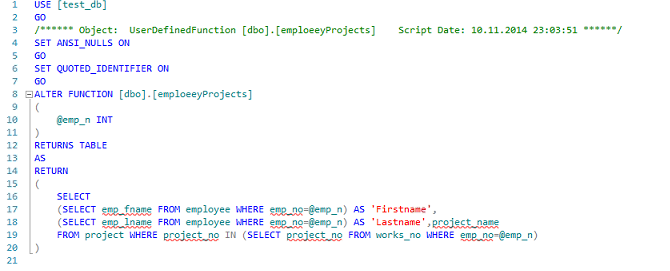
\includegraphics[scale=0.8]{FunctionsSQLServer/firstSource}}
%\caption{Re-create customers}
\end{figure}
The output of the function for argument equal 2 is like that:
\begin{figure}[H]
\centerline{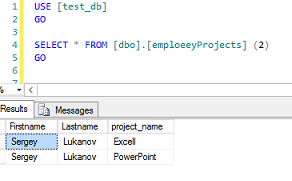
\includegraphics[scale=0.8]{FunctionsSQLServer/firstOutputFor2}}
%\caption{Re-create customers}
\end{figure}

\subsection{The second function}
The second task was the most advanced one, which I have made during whole the course, because it requires to use two cursors at the same time.The code you can see below.\\\\
 There is also very tricky moment with string summering, because the statements like a=a+b does not work, but a=b+a works well and actually return the output which should be produced by the first kind of statements.
\begin{figure}[H]
\centerline{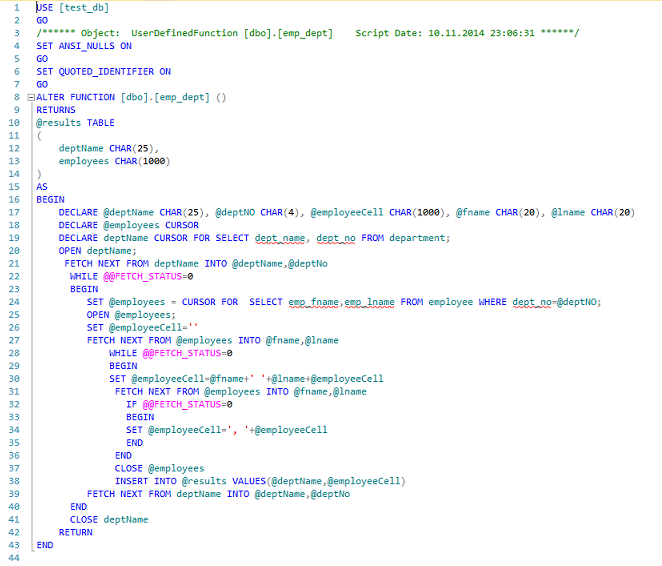
\includegraphics[scale=0.8]{FunctionsSQLServer/secondSource}}
%\caption{Re-create customers}
\end{figure}
\begin{figure}[H]
\centerline{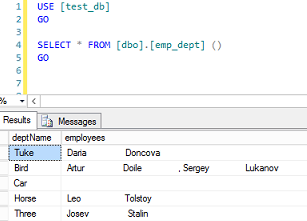
\includegraphics[scale=0.8]{FunctionsSQLServer/secondOutput}}
%\caption{Re-create customers}
\end{figure}
The output of the function follows task requirements.
\subsection{The third function}
The third task was really easy and the code is very short.
\begin{figure}[H]
\centerline{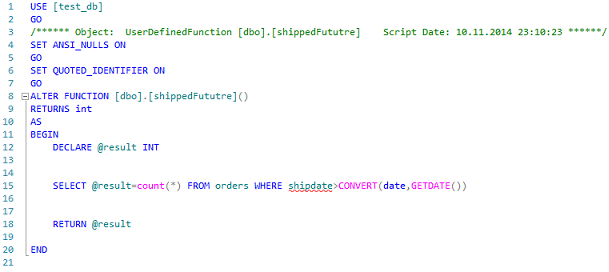
\includegraphics[scale=0.8]{FunctionsSQLServer/thirdSource}}
%\caption{Re-create customers}
\end{figure} 
And the output is correct.
\begin{figure}[H]
\centerline{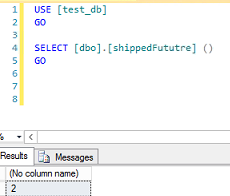
\includegraphics[scale=0.8]{FunctionsSQLServer/thirdOutput}}
%\caption{Re-create customers}
\end{figure}

\newpage
\section{Tables}
\begin{figure}[H]
\centerline{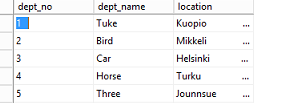
\includegraphics[scale=0.8]{FunctionsSQLServer/department}}
\caption{department table}
\end{figure}
\begin{figure}[H]
\centerline{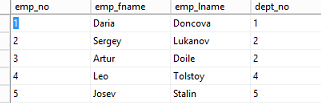
\includegraphics[scale=0.8]{FunctionsSQLServer/employee}}
\caption{employee table}
\end{figure}
\begin{figure}[H]
\centerline{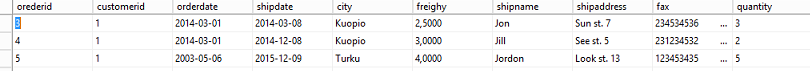
\includegraphics[scale=0.8]{FunctionsSQLServer/orders}}
\caption{orders table}
\end{figure}
\begin{figure}[H]
\centerline{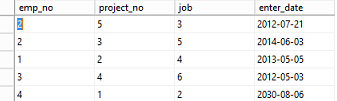
\includegraphics[scale=0.8]{FunctionsSQLServer/works_no}}
\caption{works\_no}
\end{figure}


\end{document}
